
\subsection{Non-parametric Mixture of Multivariate Normals}
\label{method:npprobitnorm}

I do not regard this as a viable model.

Note that ${\bf V}$ is the projection of the Generalized Pareto after marginal standardization
  mentioned previously onto the unit hypersphere on $L_{\infty}$.  From this, we see
  $V_{i}\in [0,1]$, $\max_i V_i = 1$. I had a thought regarding this wondering how well a simple
  Normal-Normal model would recover the original distribution, when each observation is cast into
  probit space.  That is, $W_i = \text{Probit}(V_i)$, where
  $\text{Probit}(\cdot) = \Phi^{-1}(\cdot)$, with $\Phi(\cdot)$ the CDF of a standard normal
  distribution.  This transformation pushes ${\bf V} \in [0,1]$ to ${\bf W} \in \mathcal{R}^{d}$.
  As far as why this is not a viable model, $W$ has $d$ degrees of freedom, where it should only
  have $d-1$.

As every observation $V$ has potentially some $V_i = 0$ and one $V_i = 1$, under this
  transformation these values would become $-\infty$ and $\infty$.  This would not be possible to
  fit under the normal model, so I jitter these observations by some $\epsilon > 0$ such that
  $\min V_i^{\prime} = \epsilon$, and $\max V_i^{\prime} = 1 - \epsilon$, and
  $W_i = \text{Probit}(V_i^{\prime})$.  Thus, the model becomes

\begin{equation}
  \begin{aligned}
    W_i &\sim \mathcal{N}_d\left(\mu_i, \Sigma_i\right)\\
    \mu_i, \sigma_i &\sim G_i\\
    G_i &\sim \text{DP}(\eta, G_0(\mu_i,\Sigma_i\mid\mu_0,\Sigma_0))\\
    &\hspace{1cm}G_0(\mu_i,\Sigma_i\mid\mu_0,\Sigma_0) &=
        \mathcal{N}_d(\mu_i\mid\mu_0,\Sigma_0)\text{IW}(\Sigma\mid\nu,\psi)\\
    \mu_0 &\sim \mathcal{N}_d\left({\bf u},{\bf S}\right)\\
    \Sigma_0 &\sim \text{IW}(\nu_0,\psi_0)\\
    \eta &\sim \text{Ga}(\alpha, \beta)
  \end{aligned}
\end{equation}

The updates to $\mu_i$, $\mu_0$, $\Sigma_i$, and $\Sigma_0$ are thus known forms;
  $\mu_i\mid\mu_0,{\bf W}$ and $\mu_0\mid\mu_i$ follow multivariate normal distributions.
  $\Sigma_i\mid{\bf W}$ and $\Sigma_0\mid\mu_i,\mu_0$ follow inverse Wishart distributions.

As stated, this model results in a distribution with $d$ degrees of freedom, whereas it should
  properly have $d-1$.  To generate the posterior predictive distribution and induce this $d-1$
  degrees of freedom, I cast the generated observations back to the hypercube.  That is,

  \begin{equation*}
    {\bf V}^{\text{new}} = \frac{\Phi({\bf W^{\text{new}}})}{\max_i{\bf W_i^{\text{new}}}}.
  \end{equation*}

\begin{figure}[h!]
  \label{fig:dpnormal}
  \centering
  \caption{Dirichlet Process Mixture Model with multivariate normal kernel over probit space cast
            on unit hypercube using declustered IVT dataset}
  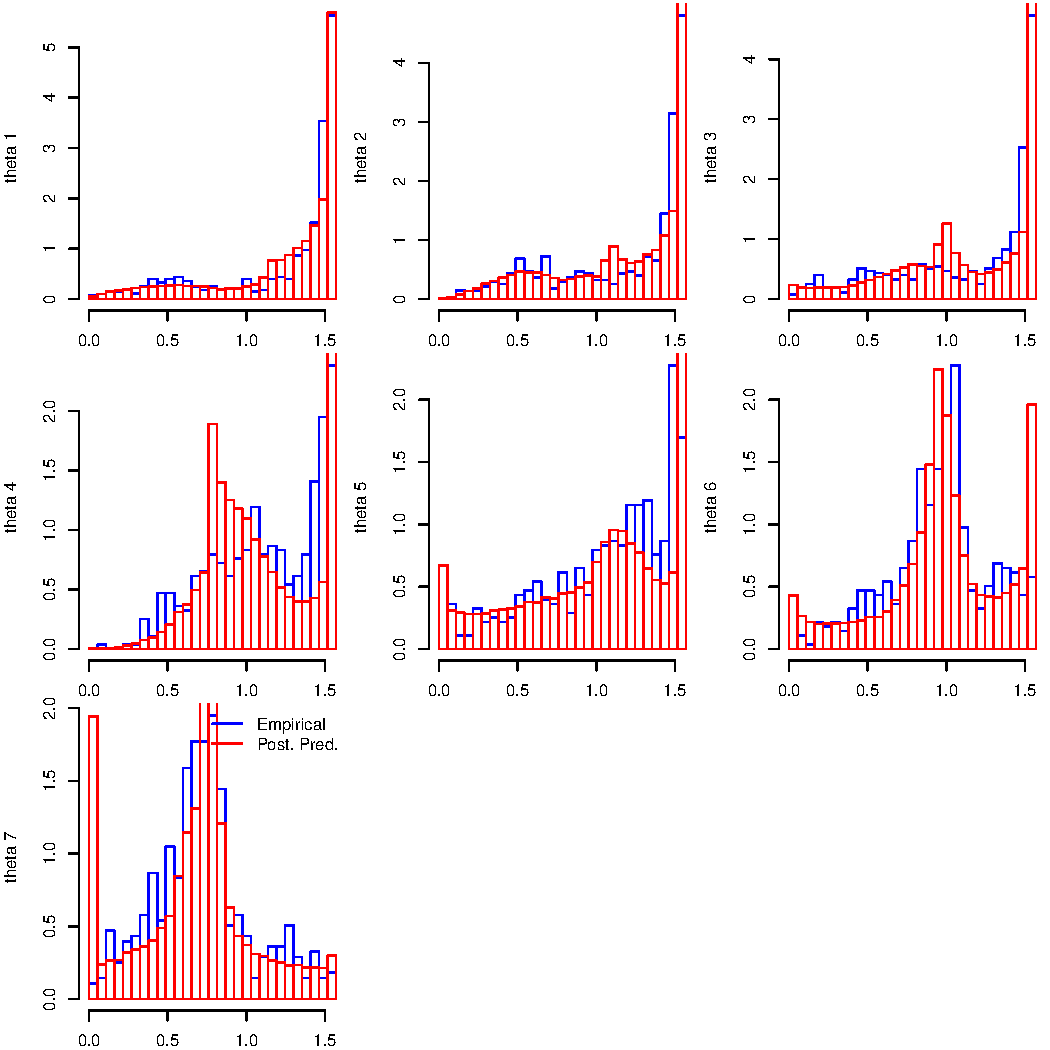
\includegraphics[width=6in]{./images/dpmp_emp_v_pred_decluster}
\end{figure}

In Figure~\ref{fig:dpnormal}, we see the resulting posterior predictive distribution, after
  casting back to the angular space.  In the Marginal $\theta$'s, this model captures pretty well
  the spikes in $\theta_6$, $\theta_7$ that have thus far confounded the mixture of projected
  gammas model.  However, it adds an unwarranted spike in $\theta_4$ and less so in $\theta_3$.
  In $\theta_6$, we also see a strong tendency towards the upper end of the range that is not
  evident in the original data.  In $\theta_7$, we see the reverse.  Odd.

\subsubsection{Casting ${\bf \theta}$ to Probit space directly}
\label{method:npprobitnorm2}

Given that the previous model had $d$ degrees of freedom, whereas by construction we need a model
  with $d-1$ degrees of freedom.  When we look at the angular representation used in the projected
  Gamma model, that gives a $(d-1)$-dimensional representation of the data, with each
  $\theta_i \in [0,\pi/2]$. It stands to reason, that we can represent this in $[0,1]$ by dividing
  the vector by $\pi/2$, and, as before, cast this into probit space.  Then we build the same
  normal-normal model used above, directly on this probit space.  This results in one of the more
  compelling models thus far.

\begin{figure}[h!]
  \label{fig:dpnormal2}
  \centering
  \caption{Dirichlet Process mixtue model with multivariate normal kernel over probit space cast
            on angular representation using declustered IVT dataset}
  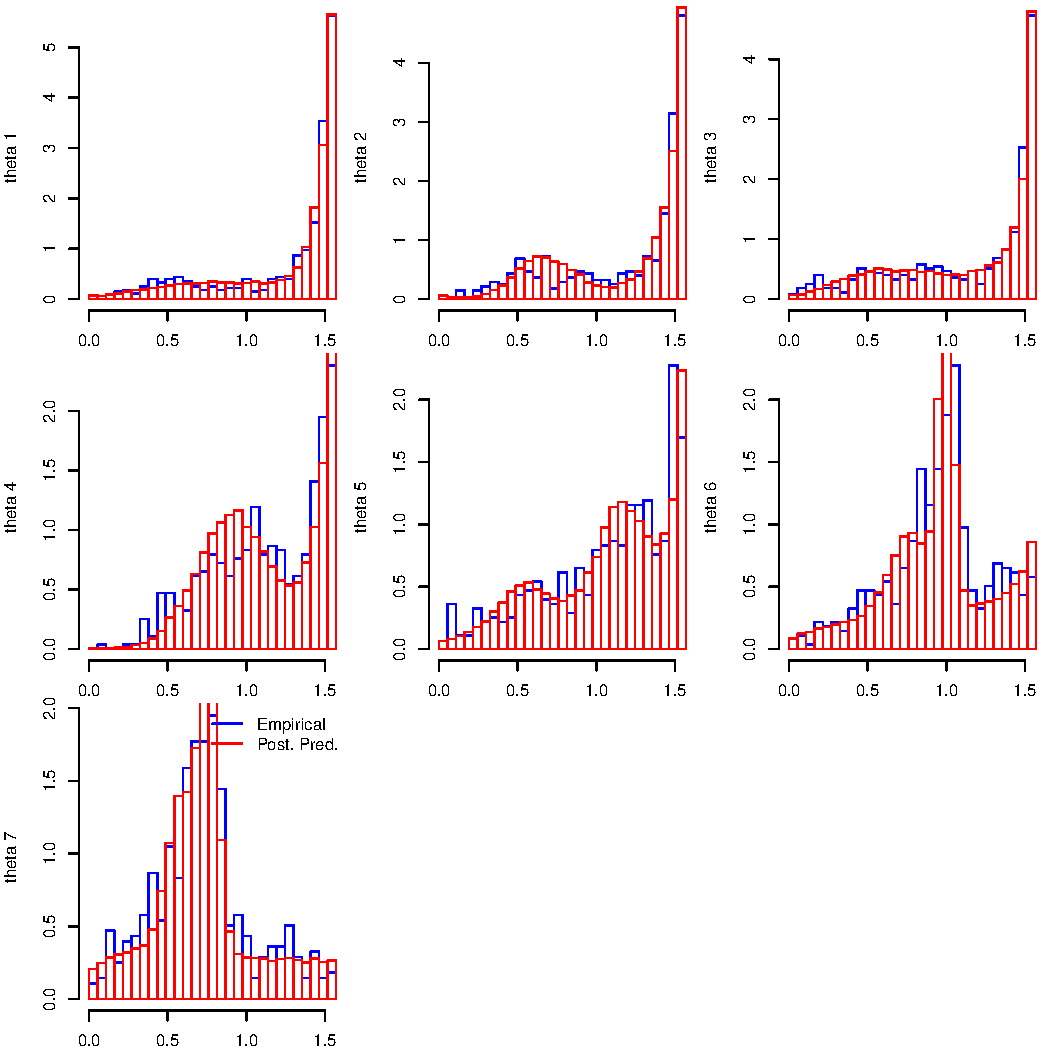
\includegraphics[width=6in]{./images/dpmp2_emp_v_pred_decluster}
\end{figure}

In Figure~\ref{fig:dpnormal2}, we see the resulting posterior predictive distribution after fitting
  on the declustered IVT data.  The resulting model is able to pick up the spikes in the later
  $\theta$'s that the mixture of projected gammas model was unable to account for.  It also does
  not exhibit the strange edge behavior in the later $\theta$'s of the previous normal model.  We
  might ask for a more granular model, as it appears that this model has been unable to fit some of
  the smaller nuances of the data, but that can likely be solved via prior specifications on $\eta$,
  $\Sigma$, and $\mu$.


% EOF
